\documentclass[a4paper,11pt]{article}

\usepackage[utf8]{inputenc}
\title{ARC1 - TP 3}
\author{Aurélien Anne, Léo Noël-Baron \& Thierry Sampaio}
\date{16/10/2015}

\usepackage{a4wide}
\usepackage{textcomp}
\usepackage[utf8]{inputenc}
\usepackage[T1]{fontenc}
\usepackage[francais]{babel}

\usepackage{graphicx}
\usepackage[usenames,dvipsnames]{color}

\usepackage{hyperref} \urlstyle{sf}
\hypersetup{
  colorlinks=true,
  urlcolor=BlueViolet,
  citecolor=BlueViolet,
  linkcolor=BlueViolet,
}
\DeclareUrlCommand\email{\urlstyle{sf}}

\newenvironment{keywords}
  {\description\item[\bsc{Mots-clés}]~$\cdot$~ }
  {\enddescription}
\newenvironment{remarque}
  {\description\item[\bsc{Remarque} ---]\sl}
  {\enddescription}
\renewcommand{\thefootnote}{\arabic{footnote}}

\usepackage{listings}
\lstset{
  language=C,
  basicstyle=\ttfamily,
  keywordstyle=\color{OliveGreen},
  stringstyle=\color{Bittersweet},
  showstringspaces=false,
  commentstyle=\color{Gray},
  numbers=left,
  numberstyle=\ttfamily\color{Gray},
  frame=l,
  columns=fullflexible,
  rulecolor=\color{Gray},
  tabsize=4,
  extendedchars=true,
  literate=
	{É}{{\'E}}1 {è}{{\`e}}1 {à}{{\`a}}1 {È}{{\`E}}1 {À}{{\`A}}1 {ê}{{\^e}}1 {â}{{\^a}}1 {î}{{\^\i}}1 {ô}{{\^o}}1
	{Ê}{{\^E}}1 {Â}{{\^A}}1 {Î}{{\^I}}1 {Ô}{{\^O}}1 {Û}{{\^U}}1 {ë}{{\"e}}1 {ï}{{\"\i}}1 {ü}{{\"u}}1 {Ë}{{\"E}}1
	{Ï}{{\"I}}1 {Ü}{{\"U}}1 {û}{{\^u}}1 {ç}{{\c c}}1 {Ç}{{\c C}}1 {æ}{{\ae}}1 {Æ}{{\AE}}1 {œ}{{\oe}}1 {Œ}{{\OE}}1
	{é}{{\'e}}1,
}
\lstMakeShortInline{|}

\parskip=0.3\baselineskip
\sloppy

\makeatletter
  \let\runtitle\@title
  \let\runauthor\@author
\makeatother

\usepackage{fancyhdr}
\pagestyle{fancy}
\fancyhead{}
\lhead{\runtitle}
\rhead{\runauthor}
\setlength{\headheight}{13.6pt}

\usepackage{amssymb}

\setlength{\parindent}{0em}
\usepackage{array}

\begin{document}

\maketitle

\subsection*{Additionneur de trois opérandes}

Le résultat d'une addition de trois opérandes sur 4 bits est compris dans l'intervalle $[0, 45]$ soit $[0, 101101]$ en binaire ; il doit donc être codé sur 6 bits. On obtient les 4 bits faibles du résultat en enchaînant deux additionneurs à deux opérandes, et on les 2 bits restants respectent la table suivante :
\begin{table}[h]\centering
\begin{tabular}{c|c}
$r_1r_2$ & $s_5s_4$ \\
00 & 00 \\
01 & 01 \\
10 & 01 \\
11 & 10
\end{tabular}\end{table}

où $r_1$ et $r_2$ sont les restes respectifs du premier et du deuxième additionneur. Ainsi on a $s_5=r_1\cdot r_2$ et $s_4=r_1\oplus r_2$, ce qui permet de concevoir le circuit en Figure \ref{add3}.

\begin{figure}[h]
\center
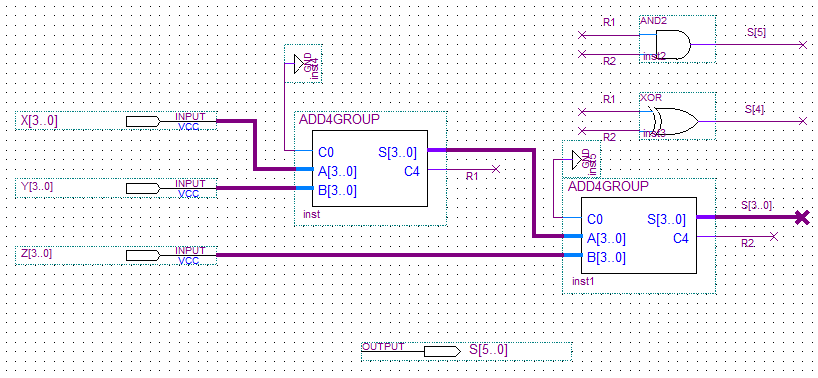
\includegraphics[scale=0.6]{add3.PNG}
\caption{Schéma du composant ADD3}
\label{add3}
\end{figure}


\subsection*{Nombre de bits à 1}

Le résultat étant compris dans l'intervalle $[0, 4]$, 3 bits suffisent pour le coder. La table booléenne correspondant à cette fonction est :
\begin{table}[h]\centering
\begin{tabular}[center]{c|c|c|c|c|c|c|c|c|c|c|c|c|c|c|c|c}
$x_3$&0&0&0&0&0&0&0&0&1&1&1&1&1&1&1&1 \\
$x_2$&0&0&0&0&1&1&1&1&0&0&0&0&1&1&1&1 \\
$x_1$&0&0&1&1&0&0&1&1&0&0&1&1&0&0&1&1 \\
$x_0$&0&1&0&1&0&1&0&1&0&1&0&1&0&1&0&1 \\ \hline
$C$&00&01&01&10&01&10&10&11&01&10&10&11&10&11&11&100
\end{tabular}\end{table}

(Pour tous les résultats à part le dernier, le bit de poids fort nul n'est pas noté par souci de place.) Cette table donne les expression booléennes suivantes pour $C = c_2c_1c_0$, qui donnent le circuit présenté en Figure \ref{nb1} :
\begin{itemize}
  \item $c_2=x_3x_2x_1x_0$
  \item $c_1=x_3\cdot\overline{x_2}\cdot\overline{x_1}\cdot x_0 + x_3x_2x_1\overline{x_0} + \overline{x_3}(x_2\oplus x_1)x_0 + \overline{x_3}x_2x_1 + x_3(x_2\oplus x_1)$
  \item $c_0=\overline{x_3}\cdot\overline{x_2}\cdot(x_1\oplus x_0) + (x_3\oplus x_2)\cdot\overline{x_1}\cdot\overline{x_0} + x_3x_2(x_1\oplus x_0) + (x_3\oplus x_2)x_1x_0$
\end{itemize}

\begin{figure}[h]
\center
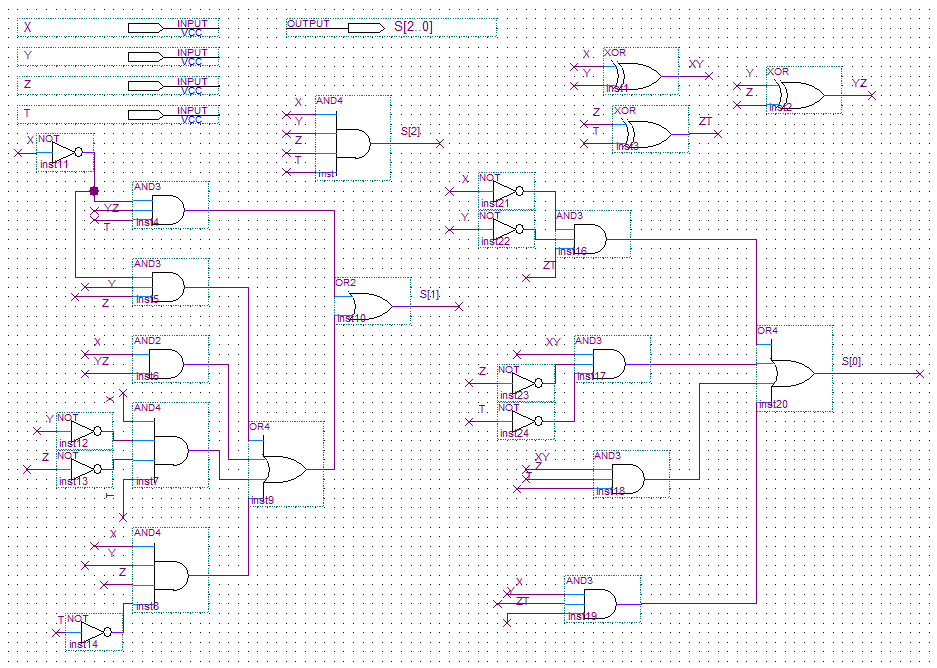
\includegraphics[scale=0.6]{nb1.PNG}
\caption{Schéma du composant NB1}
\label{nb1}
\end{figure}


\subsection*{Comparateur binaire}

L'expression formelle du comparateur sur 1 bit CMP1 est immédiate : $S=(X\oplus Y)X$ et $I=(X\oplus Y)Y$ ; ceci permet de réaliser le circuit en Figure \ref{cmp1}. Le circuit d'expansion montré en Figure \ref{expn} se conçoit en constatant qu'avec $X=X_1X_0$ et $Y=Y_1Y_0$, $X>Y\Leftrightarrow X_1>Y_1$ ou ($X_1=Y_1$ et $X_0>Y_0$), et symétriquement pour $X<Y$. Par suite, il suffit d'organiser ces deux composants comme en Figure \ref{cmp4} pour obtenir un comparateur binaire sur 4 bits.

\begin{figure}[h]
\center
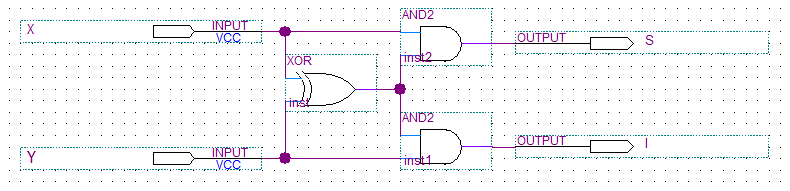
\includegraphics[scale=0.6]{cmp1.PNG}
\caption{Schéma du composant CMP1}
\label{cmp1}
\end{figure}

\begin{figure}[h]
\center
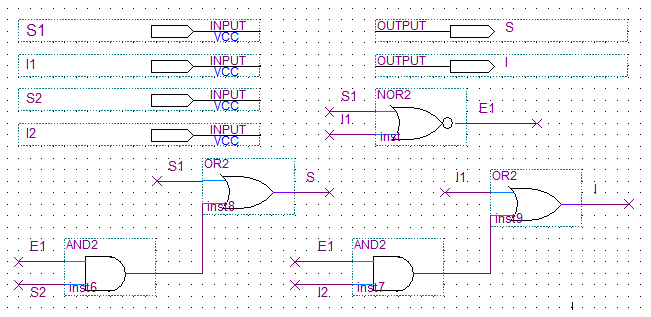
\includegraphics[scale=0.6]{exp2.PNG}
\caption{Schéma du composant EXPN}
\label{expn}
\end{figure}

\begin{figure}[h]
\center
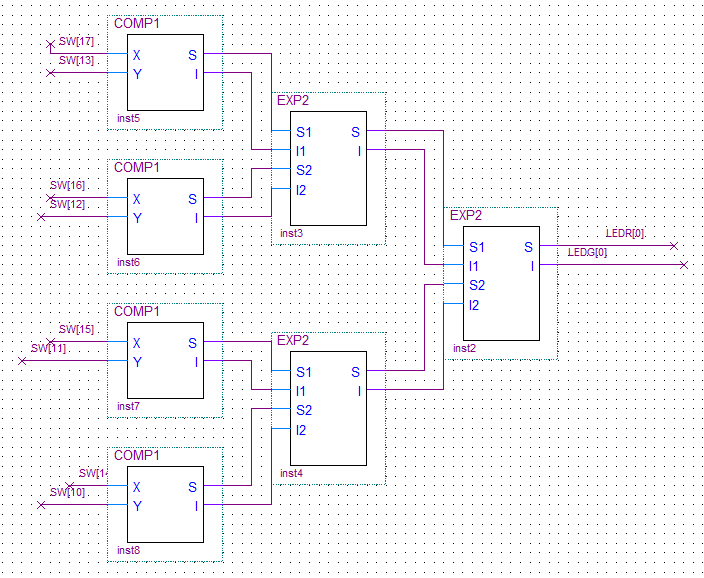
\includegraphics[scale=0.6]{cmp4.PNG}
\caption{Schéma du composant CMP4}
\label{cmp4}
\end{figure}

\end{document}
